\documentclass[12pt]{report}

\setcounter{tocdepth}{4}
\setcounter{secnumdepth}{4}

\usepackage[T1]{fontenc}
\usepackage[utf8]{inputenc}
\usepackage{polski}

\usepackage{setspace} 
\linespread{1.2}

\usepackage{geometry}              
\geometry{a4paper}                   

\usepackage{indentfirst} 	
\usepackage{afterpage}

\newcommand\blankpage{%
    \null
    \thispagestyle{empty}%
    \addtocounter{page}{-1}%
    \newpage}
    
\usepackage{hyperref}		

\usepackage{xcolor}

\usepackage{listings}		
 
\definecolor{codegreen}{rgb}{0,0.6,0}
\definecolor{codegray}{rgb}{0.5,0.5,0.5}
\definecolor{codepurple}{rgb}{0.58,0,0.82}
\definecolor{backcolour}{rgb}{0.95,0.95,0.92}
\definecolor{yellow_back}{rgb}{0.95,0.95,0.6}
\definecolor{pink_back}{rgb}{0.98,0.87,0.89}

\newcommand{\code}[1]{\colorbox{backcolour}{\texttt{\normalsize #1}}} 

\lstdefinestyle{mystyle}{
    backgroundcolor=\color{backcolour},   
    commentstyle=\color{codegreen},
    keywordstyle=\color{magenta},
    numberstyle=\tiny\color{codegray},
    stringstyle=\color{codepurple},
    basicstyle=\footnotesize,
    breakatwhitespace=\texttt{false},         
    breaklines=\texttt{true},                 
    captionpos=b,                    
    keepspaces=\texttt{true},                 
    numbers=left,                    
    numbersep=5pt,                  
    showspaces=\texttt{false},                
    showstringspaces=\texttt{false},
    showtabs=\texttt{false},                  
    tabsize=2
}
\lstset{style=mystyle}

\usepackage{tikz} 
\usepackage{pgfplots}		
\usetikzlibrary{datavisualization}
\usetikzlibrary{datavisualization.formats.functions}

\usepackage{graphicx}
\graphicspath{ {pic/} }

\usepackage[font=small,labelfont=bf]{caption}

\usepackage{amssymb}
\usepackage{epstopdf}
\usepackage{amsmath}
\DeclareGraphicsRule{.tif}{png}{.png}{`convert #1 `dirname #1`/`basename #1 .tif`.png}

\renewcommand{\maketitle}{

\begin{titlepage}
\begin{spacing}{1.0}
\begin{center}
\textbf{{\large Uniwersytet Jagielloński w Krakowie}}\\[0.5cm]
{\large Wydział Fizyki, Astronomii i Informatyki Stosowanej}\\[4cm]	
\textbf{{\Large Paweł Salwa}}\\[0.5cm]
{\normalsize Numer indeksu: 1113750}\\[2cm]
\textbf{{\LARGE 
Zastosowanie sztucznej inteligencji\\
na przykładzie gry strategicznej\\[.4cm]
}}

{\normalsize Praca licencjacka\\
na kierunku Informatyka}\\[4cm]
\begin{flushright}
{\normalsize Opiekun pracy licencjackiej:\\
dr Jan K. Argasiński\\
Zakład Technologii Gier}\\[1.0cm]
\end{flushright}
Kraków 2019
\end{center}
\end{spacing}

\thispagestyle{empty}
\noindent 

\pagebreak

\textbf{Oświadczenie autora pracy}\\
 
{\small 
\noindent
Świadom odpowiedzialności prawnej oświadczam, że niniejsza praca dyplomowa została napisana przeze mnie samodzielnie i nie zawiera treści uzyskanych w sposób niezgodny z obowiązującymi przepisami.\\
\\
\noindent
Oświadczam również, że przedstawiona praca nie była wcześniej przedmiotem procedur związanych z uzyskaniem tytułu zawodowego w wyższej uczelni.\\
\\
\noindent
Kraków, dnia \hfill Podpis autora pracy}\\
\\
\\
\\
\\
\\
\noindent 
\textbf{Oświadczenie kierującego pracą}\\

{\small
\noindent
Potwierdzam, że niniejsza praca została przygotowana pod moim kierunkiem i kwalifikuje się do przedstawienia jej w postępowaniu o nadanie tytułu zawodowego.\\
\\
\\
\noindent
Kraków, dnia \hfill Podpis kierującego pracą}
\thispagestyle{empty}

%\afterpage{\blankpage}

\end{titlepage}
}

\makeatletter

\def\@makechapterhead#1{	
  \vspace*{10\p@}			
  {\parindent \z@ \raggedleft \normalfont
    \ifnum \c@secnumdepth >\m@ne
        \@chapapp\space \thechapter
        \par\nobreak
        \vskip 0\p@			
    \fi
    \interlinepenalty\@M
    \Huge \bfseries #1\par\nobreak			
    \vskip 20\p@
    \hrule					
    \vskip 80\p@				
  }}

\makeatother

\begin{document}
\maketitle
%======================================title=================================================
\tableofcontents
\chapter {Gry RTS - strategie czasu rzeczywistego}


%======================================wstęp======================================
\section {Wstęp}
Niniejsza praca porusza problem podejmowania podstawowych decyzji przez sztuczną inteligencję w komputerowej grze strategicznej czasu rzeczywistego. 

Dołączony jest do niej projekt, który uwidacznia ten problem oraz jest przykładem implementacji jego rozwiązania. W pracy tej zostanie opisane działanie projektu oraz użyte technologie. Rozpatrzone zostaną również inne możliwe implementacje i podejścia do tego zagadnienia z teoretycznego punktu widzenia.

Sama gra zaprojektowana jest bardzo generycznie. Używa ona powszechnych mechanik, często spotykanych w swoim gatunku.


\section {Gatunek RTS}
Gry strategiczne czasu rzeczywistego - RTS (ang. real time strategy) - gatunek gier, gdzie gracza do zwycięstwa prowadzą decyzje strategiczne, a wszystkie one muszą zostać podjęte w ograniczonym czasie rzeczywistym, na bieżąco podczas rozgrywki. Gry tego typu najczęściej zostają stworzone na trzy sposoby: 
\begin{itemize}
\item[--] jako symulacje bitew i wojen z widokiem ,,z lotu ptaka", gdzie gracz zarządza jednostkami, wydając im rozkazy. Bitwy takie są zwykle urozmaicane przez nadanie jednostkom unikalnych umiejętności oraz zróżnicowanie efektywności różnych rodzajów oddziałów względem siebie (np. oddział średniowiecznej konnicy jest efektywny przeciwko łucznikom jednocześnie będąc łatwo pokonanym przez pikinierów). Dodatkowo stosuje się różne, niezależne od mechaniki bitew misje i kampanie, aby urozmaicić rozgrywkę i wpłynąć pozytywnie na odczucia gracza (w produkcji oprogramowania tzw. "user experience").
\item[--] jako symulacje ekonomiczne - w tym przypadku mamy do czynienia z zaimplementowaniem przeróżnych modeli ekonomicznych i zasad rynkowych, gdzie gracz poprzez inwestycje i handel jest w stanie pomnażać majątek, surowce i wszelakie inne zmienne liczbowe lub zdobywać zadane przez twórców osiągnięcia. Przykładem takich modeli mogą być zasady giełdy lub zależności krzywych popytu i podaży dla różnych surowców. Gry takie również często posiadają widok ,,z lotu ptaka" na mapę ekonomiczną, jednak kluczowy jest w nich interfejs, na którym twórcy muszą przejrzyście przedstawić całą gamę zmiennych zależnych od siebie oraz umożliwić przyjazną użytkownikowi interakcję z wirtualnym rynkiem.
\item[--] jako kombinacja dwóch powyższych - w grach takich stosuje się zwykle mniejszy interfejs dotyczący części ekonomicznej, a większą część ekranu zajmuje pole bitwy. Gracz jednocześnie musi podejmować decyzje dotyczące ekonomii, a jednostki i bitwy ich dotyczące mogą być traktowane zwykle jako jedna ze zmiennych ekonomicznych - inwestycja w wojsko.
\end{itemize} 
Niniejsza praca powstała na podstawie amatorskiej gry strategicznej, która jest symulacją bitwy pomiędzy jednym graczem, a komputerem. Pominąłem w niej aspekty gier RTS takie jak: makrozarządzanie, technologia, rozbudowa, scouting. Zajmę się natomiast w szczególności tematem mikrozarządzania jednostkami. 
\section {Mikrozarządzanie jednostkami} 
Jest to jedno z wielu możliwych zadań dla gracza gry RTS. Polega ono na tym, aby tak wydawać polecenia jednostkom, żeby uzyskać z nich jak największe wartości sprzyjające celom danej gry. Rodzaje tych poleceń są ściśle związane z konkretną mechaniką danej gry. Różne systemy walki mogą wymagać bardzo różnych rodzajów rozkazów. Podstawowymi, wspólnymi dla wszyskich niemalże gier dostępnymi akcjami są nakazy poruszania się oraz ataku. Często polega to na zaznaczeniu danej jednostki lub grupy jednostek i kliknięciu na cel ruchu lub ataku. Rozmieszczenie jednostek na polu bitwy skutkuje w różnej ich wartości bojowej a także przewadze strategicznej. Bardzo popularnym czynnikiem dodającym wysokich poziomów skomplikowania gry jest nadanie jednostkom unikalnych zdolności. Te z kolei mogą być: 

\begin{itemize}
\item[--] pasywne - przez ciągły wpływ na różne zmienne, mogą wpływać na wyniki bitew, a tym samym pośrednio na decyzje graczy
\end{itemize} 
oraz:
\begin{itemize}
\item[--] aktywne - wymagają bezpośredniej akcji gracza - kolejnego konkretnego rodzaju rozkazu, który urozmaica strategie i wyniki walki 
\end{itemize} 

Zdolności takie są szczególnie wymagające i udowadniają, że poza strategicznymi aspektami bitwy, można do gry dodać także aspekty takie jak: zręczność lub refleks wymagane od gracza.

Innym popularnym czynnikiem komplikującym wyniki bitew jest przewaga danego rodzaju jednostki nad innym. Jeżeli zarówno gracz jak i jego przeciwnik posiadają kilka rodzajów jednostek oraz obaj próbują zaatakować wykorzystując tę przewagę, to pole bitwy staje się bardzo skomplikowaną ,,szachownicą" podatną na tzw. ,,efekt motyla". Jest to sytuacja, w której możemy spodziewać się bardzo rozległych wyników końcowych w zależności od relatywnie małej zmiany danych początkowych. Zróżnicowanie jednostek może być bardzo łatwo implementowane, jednak wymaga ono odpowiednio ustawionych powiązanych wartości liczbowych. Zmienne te można balansować przy pomocy sukcesywnego testowania lub obliczyć dzięki modelom matematycznym. Docelowo to rozwiązanie może bardzo pozytywnie wpłynąć na wspomniane wcześniej ,,user experience" (odczucia gracza).

Atak może być w różnych scenariuszach mniej lub bardziej skuteczny a podejmowanie decyzji o wydawaniu poszczególnych rozkazów należą do graczy lub sztucznej inteligencji. Gracze muszą wydawać rozkazy w czasie rzeczywistym, a komputer ma za zadanie na bieżąco analizować dane i reagować odpowiednimi decyzjami.

Jako, że gra może pominąć niektóre popularne aspekty gier RTS, projekt będący częścią niniejszej pracy skupia się szczególnie na problemie pozycjonowania jednostek przez algorytm sztucznej inteligencji w czasie rzeczywistym jako odpowiedź na decyzje gracza. Pominięte zostaną wszelakie systemy ekonomiczne oraz rozważania dotyczące używania unikalnych zdolności jednostek.
%====================================== AI W RTS ======================================
\section {Sztuczna inteligencja w grach RTS}
Podczas projektowania AI w grach często spotykanym rozwiązaniem jest tworzenie systemu, który niekoniecznie symuluje decyzje człowieka ale raczej skupia się na odczuciach gracza i pozytywnym odbiorze gry przez niego. Okazuje się to szczególnie uproszczone przy zastosowaniu drzew decyzyjnych. Współczesne silniki posiadają wbudowane narzędzia do implementacji tego typu rozwiązań oraz całą gamę assetów i narzędzi utworzonych przez społeczność game developerską. Sprawdza się to głównie dlatego, że bardzo łatwo wyobrazić sobie i zasymulować decyzje komputera przy pomocy maszyny stanów. Drzewa decyzyjne umożliwiają łatwą implementację zachowań dla różnych stanów oraz przejść pomiędzy nimi na podstawie zmiennych w czasie rzeczywistym warunków.

Ze strony programistycznej zadanie twórców sztucznej inteligencji polega przede wszystkim na zaimplementowaniu różnych rodzajów rozkazów zaprojektowanych wcześniej przez twórców gry. Następnym krokiem jest implementacja podejmowania decyzji przez AI. Nasz komputer ma za zadanie podjąć optymalną decyzję i następnie wydać odpowiedni rozkaz. W grach typu RTS zaimplementowane muszą zostać (zależne lub niezależne od siebie) oddzielne rodzaje algorytmów do: 

\begin{itemize}
\item[--] poruszania się jednostkami - te dotyczą analizy pozycji wrogów - w praktyce obliczenia z użyciem wektorów. Tutaj problem stanowi wyszukiwanie drogi (ang. pathfinding) i optymalizacja algorytmów z nim związanych. Powszechnie stosowany jest algorytm A* i różne jego modyfikacje polegające w ogólności na wyszukiwaniu najkrótszej drogi w grafie. 
\item[--] zarządzania ekonomią - te analizują zmienne reprezentujące przeróżne aspekty rynkowe mogące istnieć w grze. Podjęcie decyzji o danym rozkazie może tutaj polegać na osiągnięciu pewnych wartości - np. decyzja o podjęciu inwestycji, gdy dochody spadną, decyzja o zwiększeniu siły armii, gdy wojska przeciwnika stały się zbyt wartościowe i dla nas groźne. Mogą być one zdefiniowane wcześniej lub obliczane na bieżąco w czasie rzeczywistym na podstawie dowolnie zaimplementowanych wzorów.
\item[--] dyplomacji - np. losowo imitującej zachowania innych graczy dla lepszego UX użytkownika.
\item[--] rozwoju technologii - dotyczy podobnego problemu jak zarządzanie ekonomią. Większość gier stosuje przystępny model drzew technologicznych, gdzie wynalezienie pewnej technologii odblokowuje kolejne, bardziej zaawansowane. Tutaj implementacja może być bardzo uproszczona - polegać może na wcześniejszym zakodowaniu ścieżki poszczególnych decyzji i zczytywaniu z niej lub nawet na losowym wyborze kolejnych kroków. To ostatnie rozwiązanie możliwe jest jednak tylko, jeżeli pomiędzy różnymi krokami zachowany jest balans.
\end{itemize}


%====================================== Współczesne rozwiązania=================================
\section {Współczesne rozwiązania} 
Gdy mamy do czynienia z grą typu szachy - gdzie dwóch graczy o równych szansach startuje do walki, algorytmy AI muszą być bardzo skomplikowane i poprawnie wartościować poszczególne decyzje. Gdy gra polega raczej na przechodzeniu kolejnych misji optymalnym rozwiązaniem jest oskryptowanie każdej. Ponieważ maszyny stanów mogą bardzo dokładnie symulować pewne sekwencyjne, zdefiniowane i powtarzające się akcje, sprawdzają się one bardzo dobrze w sytuacjach, gdzie gracz jest prowadzony przez rozgrywkę według planu twórców. Dlatego też misje, mapy w grach łatwo można oskryptować według wymyślonego modelu przy pomocy drzew decyzyjnych. Dotyczy to zwykle rutynowych akcji wykonywanych przez sztuczną inteligencję. Przykładami mogą być: atak, wysłanie zwiadu, wybudowanie budynku lub zakup surowców raz na określony czas. Takie rozwiązanie jest bardzo łatwe do modelowania i testowania. Dzięki temu programista może łatwo dopasować implementację do zaprojektowanego modelu. 

Problem rośnie jednak, gdy model gry pozwala na coraz więcej możliwych decyzji do podjęcia i sztuczna inteligencja musi raczej odpowiadać na dane nawet parudziesięciokrotnie w ciągu każdej sekundy, niż egzekwować kolejne rozkazy z oskryptowanej mapy. 

Poniżej wymienienione zostały podstawowe koncepty używane współcześnie:
\begin{itemize}
\item[--] sztuczne sieci neuronowe - jest to wyjątkowe i zaawansowane rozwiązanie, które daje niezastąpione możliwości. Ich szczególną zaletą jest możliwość samodzielnego uczenia się przez program. Na chwilę obecną nie uzyskało jednak wielu zastosowań w branży produkcji gier komputerowych. Spowodowane jest to głównie nieprzewidywalnością algorytmów opartych na sieciach oraz trudnością w ich debugowaniu. Mogą być jednak użyteczne w przypadku problemów nieliniowych, które ciężko rozwiązać tradycyjnymi metodami. Głównie stosuje się je jednak w celach naukowych i hobbystycznym tworzeniu botów do istniejących gier raczej, niż w komercyjnych produkcjach. Dzięki możliwości analizy ogromnej ilości różnych strategii, sieci neuronowe okazały się być wyzwaniem nawet dla profesjonalnych graczy. Współczesne boty stworzone do grania w popularną grę strategiczną Starcraft mając okazję zmierzyć się z mistrzami świata, wciąż przegrywały zwykle, z niewielką jednak przewagą ludzi.
\item[--]  systemy oparte na zasadach - (\textbf{ang. rule based systems}) - ogólny termin określający ogólny zbiór danych i zasad ich interpretowania. Są one najobszerniej używane w programowaniu sztucznej inteligencji, zarówno w grach jak i w innych programach używających AI. Możliwości implementacji takiego systemu są nieograniczone i dają programiście duże pole do popisu. Szczególnym elementem jest tutaj silnik oparty na wnioskowaniu z danych zapisanych w pamięci. Programista może oczywiście wcześniej zaprojektować dane (np. pod podstacią klas jako kontenerów na nie). W ogólności zadaniem silnika jest podejmowanie konkretnych, optymalnych działań. W projekcie, który jest częścią niniejszej pracy skorzystałem z tego rozwiązania. Aby wnioskować w czasie rzeczywistym, algorytmy sztucznej inteligencji wywołoywane są w funkcji \texttt{\texttt{Tick}()}, a ta z kolei wywoływana jest za pośrednictwem samego silnika Unreal Engine 4.
\item[--] maszyny stanów, automaty skończone (\textbf{ang. finite state machines}) - teoretycznie można zaliczyć je do systemów opartych na zasadach, jednak obszerność zastosowania oraz ich unikalność zasługuje na odrębny opis. Zwięźle omawiając: maszyna stanów to system złożony z wielu stanów i przejść pomiędzy nimi. Elementy te, można dowolnie definiować. Każdy stan może odpowiadać za zbiór zachowań na wejściu maszyny do tego stanu, na wyjściu ze stanu oraz podczas trwania pomiędzy tymi wydarzeniami. Przejście pomiędzy stanami również można dowolnie determinować jednak najczęściej stosuje się do tego programistyczne delegaty i eventy. Jest to szczególnie przystępne rozwiązanie, kiedy mamy jasno zdefiniowany zbiór ciągłych, sekwencyjnych rodzajów zachowań AI. To możemy zaobserowować w grach typu FPS, RPG, logicznych. Maszyny te są - poza problemami związanymi z AI - powszechnie stosowane jako programistyczne modele i wzorce projektowe. Obecne silniki do gier używają ich nawet do obsługi animacji. Każda animacja jest stanem, z którego przechodzimy do kolejnych.  Przejścia pomiędzy stanami powodują tutaj mieszanie się (\textbf{ang. ,,animation blending"}) kolejnych animacji w celu płynnego, naturalnego ich wyglądu.
\end{itemize}







%======================================Zarys problemu pracy======================================
\section {Zarys problemu pracy}
Powszechną mechaniką spotykaną współcześnie w grach RTS jest regeneracja punktów życia zranionych w walce jednostek. Regeneracja odbywa się poza bitwami i zakładamy, że raz zabita jednostka, nie może się odrodzić. W związku z tą kwestią nasuwa się myśl:

\noindent\textbf{\textit{Jednostka (choćby ledwie) żywa jest więcej warta od jednostki martwej.}}

Tak więc dążymy do takiego zarządzania jednostkami, aby w trakcie bitwy zminimalizować ilość straconych jednostek, tym samym nie martwiąc się, że nasze jednostki wyjdą z bitwy ranne. Z drugiej strony w tym samym czasie, zależy nam, aby nie pozwolić na ucieczkę jednostkom przeciwnika, które są poważnie ranne. Takie zachowanie wiąże się zwykle z trzema rodzajami rozkazów:
\begin{itemize}
\item[--] ucieczka jednostek, które są zagrożone śmiercią, w kierunku przeciwnym do zagrożenia,
\item[--] skupianie ataku wielu swoich jednostek na pojedynczych jednostkach przeciwnych tak, aby zwiększyć ich zagrożenie tym samym zmniejszając czas na reakcje dla przeciwnika,
\item[--] rozmieszczenie wojsk tak, aby jednostki w swoim zasięgu walki posiadały przewagę liczebną.
\end{itemize}

Są to rozwiązania sprawdzone i stosowane przez współczesnych profesjonalnych graczy. Dotychczas zbyt przesadne - chodź wartościowe - mikrozarządzanie przez boty nie jest zaimplementowane do sztucznych inteligencji występujących we współczesnych grach  RTS. 

Ponieważ symulacje bitew w grach tego rodzaju są często uproszczone i bierze w nich udział kilkanaście do maksymalnie kilkudziesięciu jednostek, człowiek ze swoim refleksem jest w stanie efektywnie zarządzać każdą posiadaną jednostką. Jest to dopasowane do przeciętnego niepoczątkującego gracza, którego wskaźnik APM - akcji na minutę (\textbf{ang. APM - Actions Per Minute}) wynosi około 100 - 140. Warto nadmienić, że profesjonalni gracze są w stanie osiągnąć wskaźnik APM równy nawet 250. Nie wykorzystają oni jednak w tak prostej grze swojego potencjału z powodu mocno ogarniczonej ilości rodzajów rozkazów.

Problemem jest to, aby komputer wydawał rozkazy swoim jednostkom w sposób racjonalny, symulując ludzkiego przeciwnika. Celem projektu dołączonego do niniejszej pracy jest stworzenie gry, posiadającej podstawowe mechaniki zarządzaia jednostkami z gier typu RTS wraz ze sztuczną inteligencją imitującą wydawanie powyżej wymienionych rozkazów w ten sposób, aby gracz miał równe szanse z na wygraną z komputerem. Dodatkową zasadą jest to, żeby żadna ze stron nie miała przewagi z góry. W kolejnych rozdziałach rozważona zostanie implementacja tych rozkazów oraz programowanie podejmowania tych decyzji przez komputer. 

Celem pracy jest teoretyczny opis tych problemów, zaproponowanie rozwiązań oraz wyjaśnienie implementacji dołączonego projektu.

%=========================================================================================
\chapter{Użyta technologia - \\silnik Unreal Engine 4}

Unreal Engine 4 jest rzadko wykorzystywany we współczesnej branży wytwarzania gier komputerowych do tworzenia gier typu RTS. Jest to głównie podyktowane trendami. Rzadziej - lecz również - powodami związanymi z optymalizacją. Większość podstawowych assetów i szablonów projektów są przygotowane, aby dać podstawy grom poniższych typów:
\begin{itemize}
\item[--] FPS (ang. First Person Shooter) - strzelanka pierwszoosobowa,
\item[--] akcji,
\item[--] RPG (ang. Role Playing Game),
\item[--] przygodowe,
\item[--] platformowe,
\item[--] puzzle (łamigłówki logiczne),
\item[--] inne rodzaje gier z widokiem trzeciej osoby - TPP (ang. Third Person Perspective) - sportowe, symulacje lub typu ,,hack and slash".
\end{itemize}

Nie oznacza to jednak, że silnik ten nie jest lub nie może zostać wykorzystywany do gier RTS. Jedynym ograniczeniem jest wydajność, wszystkie aspekty i implementacje typowe dla tego gatunku gier jesteśmy w stanie osiągnąć używając Unreal Engine 4. 

W niniejszej pracy nie zajmowałem się tematem optymalizacji związanej z modelami 3D, a użytych zostało wiele darmowych assetów udostępnianych przez twórców silnika. Nie są one zatem poprawnie przystosowane do gry RTS. Dla uproszcznia w modelach projektu ominąłem optymalizację z systemem LOD (Ang. Level Of Detail - zmienny poziom dokładności modeli w zależności od odległości). 

Przy wielu natywnych assetach koniecznym było skorzystanie z możliwości dziedziczenia po natywnych dla silnika klasach C++. Dyktowane było to potrzebą rozszerzenia ich o funkcjonalność związaną z grami RTS, których - jak nadmieniłem wcześniej - nie posiadają podstawowe szablony silnika.


Test wydajności będzie również zawarty w niniejszej pracy.

%==================================BPBasic UNIT==========================================
\section{Asset pojedynczej jednostki}

Hierarchia dziedziczenia klas w projekcie jest zaprojektowana tak, aby użyć możliwie najwięcej poprawnych dla gier RTS rozwiązań udostępnianych przez twórców Unreal Engine 4. Jednostka - czyli zwykły ,,żołnierz" - w naszej grze, jest zapisana pod postacią obiektu \textit{BP\_BasicUnit}. Klasa tego obiektu dziedziczy po klasie \texttt{SalwaRTS.MyCharacter.h}

Ponieważ potrzebne jest, aby instancjować wiele obietów tej klasy, zgodnie z zasadą działania silnika musi być ona assetem typu Blueprint Class. Funkcjonalność tej klasy podzielona jest dzięki chierarchii dziedziczenia na dwa dedykowane dla projektu pliki: 
\begin{itemize}
\item[--] \texttt{AMyCharacter.h} - zawierającą klasę C++
\item[--] \texttt{\texttt{BP\_BasicUnit}} - klasa Blueprint umożliwiająca wielokrotne instancjowanie jednostek w poziomach w silniku
\end{itemize}

\texttt{AMyCharacter.h}- zawiera klasę dziedziczącą po unrealowej klasie \texttt{ACharacter}. Dzięki temu zachowania takie jak: ruch jednostki, atak jednostki, otrzymywanie obrażeń są już zaimplementowane przez twórców silnika. W niniejszym projekcie potrzebne było rozszerzenie jej o zachowania typowe dla gry RTS, oraz o esencje tematu pracy, czyli algorytmy sztucznej inteligencji. To klasa AMyCharacter, w pliku \texttt{AMyCharacter.cpp} zawiera implementacje wszystkich funkcji, których potrzebuje pojedyncza jednostka, aby podejmować decyzje związane ze sztuczną inteligencją.

\subsection{Klasa AMyCharacter}
Poniżej widoczny kod przedstawia pola klasy \texttt{AMyCharacter}:

\begin{lstlisting}[language=C++, backgroundcolor=\color{black!5}, basicstyle=\footnotesize, caption=Publiczne pola klasy \texttt{AMyCharacter}]
public:	
	UPROPERTY(EditAnywhere, BlueprintReadWrite, Category = Units)
	TArray<AMyCharacter*> VisibleUnits;
	UPROPERTY(EditAnywhere, BlueprintReadWrite, Category = Parameters)
	float MaxHp = 100;
	UPROPERTY(EditAnywhere, BlueprintReadWrite, Category = Parameters)
	float CurrentHp = 100;
	UPROPERTY(EditAnywhere, BlueprintReadWrite, Category = Parameters)
	float CooldownBetweenAttacks;
	UPROPERTY(EditAnywhere, BlueprintReadWrite, Category = Parameters)
	float AttackDuration;
	UPROPERTY(EditAnywhere, BlueprintReadWrite, Category = Parameters)
	float DamagePerAttack;
	UPROPERTY(EditAnywhere, BlueprintReadWrite, Category = Parameters)
	bool bHasTargetToAttack;
	UPROPERTY(EditAnywhere, BlueprintReadWrite, Category = Parameters)
	bool bIsAttacking;
	UPROPERTY(EditAnywhere, BlueprintReadWrite, Category = Parameters)
	bool bCanAttack;
	UPROPERTY(EditAnywhere, BlueprintReadWrite, Category = Parameters)
	bool bIsAlive;
\end{lstlisting}

Pola te są opatrzone makrami, które silnik wykorzystuje do odpowiedniej serializacji danych pomiędzy kodem, a samym edytorem. Jest to bardzo ważne, ponieważ dziedzicząca klasa Blueprint \texttt{BP\_BasicUnit} musi mieć do nich dostęp, aby implemenotwać własną funkcjonalność w języku Blueprint. Zastosowanie poszczególnych pól jest następnujące:
\begin{itemize}
\item[--] \texttt{TArray<AMyCharacter*> VisibleUnits}; - Kluczowa tablica dynamiczna, służąca do przechowywania wszystkich jednostek przeciwnika, które są w zasięgu. Jest ona uzupełniana za każdym razem, gdy system kolizji w silniu wykryje kolizję niewidocznych sfer, które są przymocowane jako komponenty do każdej jednostki i odpowiadają za wykrywanie czy jednostki te stanowią dla siebie nawzajem zagrożenie. Tablica ta wykorzystywana jest w funkcjach algorytmu sztucznej inteligencji, aby znajdować środek zagrożenia oraz szacowany czas, jaki jednostka jest w stanie przetrwać przed śmiercią.
\item[--] \texttt{MaxHp}, \texttt{CurrentHp}, \texttt{CooldownBetweenAttacks}, \texttt{AttackDuration}, \texttt{DamagePerAttack} - te zmienne typu float zdefiniowane są według zasady samodokumentującego się kodu i po przetłumaczeniu ich nazw jasno jest określone do czego używane są wartości, które przechowują. Regulują one podstawowe wielkości, które dzięki makrom silnika możemy edytować z poziomu edytora. Ten sposób projektowania jest pomocny na etapie tworzenia projektu, ponieważ nie trzeba kompilować całego kodu, aby uruchomić grę na innych ustawieniach. Może być to szczególnie przydatne, gdy wartości te chcemy dopasować do lepszego UX oraz do uzyskania balansu w grze.
\item[--] \texttt{bHasTargetToAttack}, \texttt{bIsAttacking}, \texttt{bCanAttack}, \texttt{bIsAlive},- zmienne typu boolean wykorzystywane przy podpinaniu animacji oraz w algorytmach związanych z wzajemnym atakowaniem jednostek.

\end{itemize}


Poniżej widoczny kod przedstawia funkcje klasy \texttt{AMyCharacter} z pliku nagłówkowego\texttt{AMyCharacter.h}: 
\begin{lstlisting}[language=C++, backgroundcolor=\color{black!5}, basicstyle=\footnotesize, caption= Funkcje klasy AMyCharacter z pliku nagłówkowego \texttt{AMyCharacter.h}]
public:
	virtual void Tick(float DeltaTime) override;
	virtual void SetupPlayerInputComponent(
	class UInputComponent* PlayerInputComponent) override;
	UFUNCTION(BlueprintPure, Category = Health)
	float GetHealthPercentage();
	UFUNCTION(BlueprintCallable, Category = Health)
	void ReceiveDamage(float Amount);
	UFUNCTION(BlueprintImplementableEvent, BlueprintCallable)
	void Attack(AMyCharacter* UnitTargetToAttack);
	UFUNCTION(BlueprintImplementableEvent, BlueprintCallable)
	void StartOfOverlap();
	UFUNCTION(BlueprintImplementableEvent, BlueprintCallable)
	void MoveTo();
	UFUNCTION(BlueprintImplementableEvent, BlueprintCallable)
	void DamageReceived(float Amount);
	UFUNCTION(BlueprintImplementableEvent, BlueprintCallable)
	void GetNewTargetToAttack();

	FVector GetMiddleOfEnemies();
	FVector GetVectorOfEscape();
	float GetCurrentEscapeTime();
	float GetCurrentEscapeRouteLength();
	float GetCurrentSurvivalTime();
	bool CheckIfShouldEscape();
	bool CheckIfCanEscape();
	void Escape();
\end{lstlisting}
Ich działanie będzie dokładnie opisane w rozdziale trzecim nieniejszej pracy, ponieważ bezpośrednio dotyczy tematu pracy i zasługuje na obszerne i odrębne wytłumaczenie.

Funkcje napisane w C++ z pliku \texttt{AMyCharacter.cpp} wywoływane są zarówno z Blueprintu \texttt{BP\_BasicUnit} jak i przez silnik. Unreal robi to za pośrednictwem funkcji \texttt{\texttt{Tick}()} wołanej przy każdej ramce oraz \texttt{BeginPlay()}, wołanej na początku rozgrywki, po włączeniu gry. Funkcja \texttt{Tick} jest natomiast punktem wyjścia dla algorytmu sztucznej inteligencji. 
\begin{lstlisting}[language=C++, backgroundcolor=\color{black!5}, basicstyle=\footnotesize, caption= Funkcje wołane przez silnik w pliku \texttt{AMyCharacter.h}]
void AMyCharacter::BeginPlay();
void AMyCharacter::Tick(float DeltaTime);
\end{lstlisting}

\subsection{Zawartość ,,Event Graph" w BP\_BasicUnit}
W niniejszym podrozdziale opisane zostaną obsługi eventów dotyczących klasy Blueprint BP\_BasicUnit. Podgląd algorytmów można otrzymać tylko otwierając plik w edytorze Unreal Engine 4. Algorytmy zawarte tutaj dotyczą obsługi kolizji, spawnowania kolejnych jednostek, animacji, ataku oraz śmierci jednostek. Jako, że każda jednostka posiada przymocowaną do siebie niewidoczną sferę, która wykrywa jednostki będące w zasięgu ataku, to przede wszystkim potrzebna jest obsługa dwóch eventów: \texttt{OnComponentBeginOverlap} i \texttt{OnComponentEndOverlap}. Obsługa ich wywołania jest następująca:
\begin{itemize}
\item[--] \texttt{OnComponentBeginOverlap} - Gdy inna jednostka zacznie kolidować z naszą, najpierw musimy sprawdzić, czy należy ona do gracza, czy do komputera. Gdy należy do tej samej drużyny, ignorujemy ją całkowicie. W przeciwnym przypadku dodajemy ją do tablicy \texttt{VisibleUnits} funkcją \texttt{AddUnique()}, która pozwala uniknąć zduplikowania tej samej jednostki w tej kolekcji i zapewnia, że każdy jej element jest unikalny. Na koniec musimy ustawić zmienną typu bool - bHasTargetToAttack na \texttt{true}, która będzie potrzebna w innych miejscach projektu do poprawnego działania algorytmów związanych z atakiem i obsługą animacji.
\item[--] \texttt{OnComponentEndOverlap} - Na końcu kolizji usuwamy kolidującą jednostke z tablicy \texttt{VisibleUnits}. Analogicznie jak w evencie OnCompoenentBeginOverlap ustawiamy zmienną \texttt{bHasTargetToAttack} - tym razem na \texttt{false} - jednak tylko, jeżeli usunięta jednostka była ostatnią w tablicy.
\end{itemize}

Podczas wywoływania powyższych eventów wywoływana jest również Blueprintowa funkcja \texttt{FindTargetToAttack()}. Odpowiada ona za znalezienie nowego celu ataku (gdy obecny cel jest odpowiedni nic się nie zmienia) i umieszczenie referencji do niech w zmiennej typu \texttt{BP\_BasicUnit} nazwanej \texttt{UnitTargetToAttack}. Jej wywołanie jest potrzebne znowu - w dwóch sytuacjach:
\begin{itemize}
\item[--] gdy obecny cel ataku zginie - wywołuje on wtedy event OnDeath. Ten z kolei jest przypisywany każdej widocznej jednostce i poza wywołaniem funkcji \texttt{FindTargetToAttack()}, nakazuje atak kolejnej jednostki (zostanie to wyjaśnione przy opisie eventu Attack)
\item[--] żywy ucieknie poza zasięg (wywoływanie następuje zawsze w evencie

\texttt{OnComponentEndOverlap}).
\end{itemize}




\section{Kontroler - dane wejściowe od gracza}
Unreal Engine 4 udostępnia klasę C++ - \texttt{PlayerController}, do zbierania danych wejściowych z urządzeń zewnętrznych i wdrożenia odpowiednich akcji przez silnik jako odpowiedź na akcje gracza. Umożliwia on obsługę przeróżnych kontrolerów, urządzeń VR, padów, ekranów dotykowych, jednak w naszym przypadku potrzebne jest tylko zebranie danych z myszki oraz klawiatury. Klasa PlayerController jest w stanie otrzymywać również powiadomienia od wszelakich wydarzeń mających miejsce w grze (tzw. event), dzięki czemu programista może wywoływać swoje funkcje od razu - jako reakcje na stan gry.

W projekcie funkcję kontrolera pełni asset \textit{CameraPawnController} dziedziczący po klasie \texttt{PlayerController}. \textit{CameraPawnController} jest rozszerzony w stosunku do \textit{PlayerController'a} o funkcje, które są potrzebne w szczególności w grze RTS. Jest w nim umieszczona pełna logika akcji, które są odpowiedzią na kliknięcia lewym, prawym oraz środkowym przyciskiem myszki, wciśnięcia przycisków na klawiaturze jak i przesuwanie myszką po oknie gry przez gracza.

Ponieważ, głównym elementem którym w grze potrzeba poruszać w zależności od danych wejściowych jest kamera - prostym rozwiązaniem jest przymocowanie kamery do obiektu klasy \textit{Pawn}. W Unreal Engine 4 obiekty tego typu są używane jako aktorzy, którzy mogą być kontrolowani przez gracza lub sztuczną inteligencję. W projekcie, funkcję takiej klasy pełni asset 'CameraPawn' dziedziczący po klasie \textit{Pawn}. W projekcie główna kamera jest komponentem tego właśnie obiektu, co oznacza, że jej relatywna pozycja, rotacja i skala względem niego pozostaje stała, niezależnie od wersji globalnej zapisanej w assecie poziomu. Ponieważ każdy obiekt, który jest umieszczony w poziomie w Unreal Engine 4 posiada komponent location, możemy dowolnie zmieniać położenie każdego z nich. Location posiada publiczne zmienne x, y, z, którymi możemy dowolnie manipulować zarówno z poziomu C++ jak i Blueprint. Jako, że kamera jest przymocowana do obiektu klasy \textit{Pawn} - a obiekt ten posiada komponent location - jeżeli chcemy zmienić pozycję kamery, wystarczy, że zmienimy położenie Pawna.

\subsection{Ruch kamery}

Klasa Blueprint CameraPawnController zawiera w sobie obsługę ruchu kamery. Odpowiedzialne są za to funkcje MovementX i MovementY. Zmieniają one wektor Location zawarty w komponencie Transform kamery odpowiednio w osiach X i Y. Szybkość tej zmiany jest zależna od dwóch zmiennych typu float: 
\begin{itemize}
\item[--] \texttt{MouseMoveMultiplier} - którą programista może dowolnie zmienić z poziommu edytora UE4
\item[--] \texttt{MoveSensitivity} - ta z kolei jest wyliczana na podstawie obecnej odległości kamery od ziemi. Odległość tą możemy otrzymać ze zmiennej TargetArmLength będącej w komponencie SpringArm. Jest ona dzielona przez 50 i następnie zatrzaskiwana pomiędzy wartością minimalną 0,5 i maksymalną 30. Podane dane liczbowe otrzymałem na podstawie prób i błędów. Ustawione są tak, aby gracz mógł swobodnie poruszać kamerą gdy jest przybliżona - tzn. gdu zmienna TargetArmLength ma relatywnie małą   wartość - wtedy prędkość poruszania się kamery jest odpowiednio mniejsza. Dzięki zatrzaśnięciu wyniku dzielenia TargetArmLength przez 50 Zapobiega zbyt wolnemu lub zbyt szybkiemu ruchowi kamery.
\end{itemize}



Funkcje MovementX i MovementY mogą być wywołane za pośrednictwem dwóch akcji:

\begin{itemize}
\item[--] przeciągnięcie kursora myszy do krawędzi ekranu - po otrzymaniu obecnej pozycji kursora - przy pomocy funkcji GetCursorPosition() - dzielimy jej poszczególne składowe przez odpowiednie składowe funkcji GetViewportSize() i następnie sprawdzamy, czy wynik dzielenia jest większy niż 0,975 lub mniejszy niż 0,025. Jeżeli sprawdzenie da wynik pozytywny, wywołujemy odpowiednią z dwóch funkcji: MovementX lub MovementY, w zależności, czy kursor jest w pobliżu krawędzi pionowych czy też poziomych. W ogólności oznacza to, że gdy kursor znajdzie się w 0,025 szerokości lub wysokości ekranu, następuje ruch kamery. 
\item[--] kliknięcie jednego spośród przycisków : 'w', 'a', 's', 'd'. W ustawieniach projektu w dziale 'input' przyciski ,,W" i ,,S" zmapowane są do jednej osi nazwanej 'MoveForward', a ,,A" i ,,D" do drugiej osi nazwanej 'MoveRight'. Do tak zmapowanych przycisków możemy odnieść się w klasach Blueprint przy pomocy eventów InputAxisMoveForward oraz InputAxisMoveRight. Event taki daje nam wartość AxisValue równą 1 lub -1 w zależności od przycisku, który wciśniemy (np. przycisk ,,W" da nam wartość 1, gdy ,,S" wartość -1). Wartość ta następnie przekazywana jest do funkcji MovementX lub MovementY i następuje ruch kamery w oczekiwanym kierunku.
\end{itemize}

Wywołania funkcji i obsługa eventów umiejscowione są w zakładce 'Event Graph' klasy Blueprint 'BP CameraPawnController'.

\subsection{Obsługa lewego przycisku myszy}

Lewy przycisk myszy obsługuje algorytm napisany w całości używając Blueprintóww w pliku 'BP CameraPawnController'. Przycisk ten jest odpowiedzialny za zaznaczanie jednostki, gdy na nią klikniemy, lub zaznaczenie wielu jednostek, gdy po kliknięciu przeciągniemy mysz - tworząc przekątną prostokąta - i następnie puścimy przycisk. Wtedy zaznaczone zostają wszystkie jednostki, których model, czyli wielościan 3d znajduje się pod tworzonym przez zaznaczenie prostokątem. Prostokąt ten jest również rysowany na ekranie i podświetlany zielonym kolorem. Do jego narysowania używany jest tutaj plik BP\_MyHUD, czyli podstawowa klasa Blueprint odpowiedzialna za UI (ang. User Interface - interfejs użytkownia). W momencie puszczenia przycisku wywoływana jest funkcja 

MyGetActorsInSelectionRectangle().
\begin{lstlisting}[language=C++, backgroundcolor=\color{black!5}, basicstyle=\footnotesize, caption=Funkcja MyGetActorsInSelectionRectangle() w klasie MyHUD.]
void AMyHUD::MyGetActorsInSelectionRectangle(
    TSubclassOf<class AActor> ClassFilter, 
    const FVector2D& FirstPoint, 
    const FVector2D& SecondPoint, 
    TArray<AActor*>& OutActors
)
\end{lstlisting}

Jest to funkcja zapisana w języku C++, wywoływana z poziomu Blueprint, dopasowana do projektu, która oryginalnie zawarta jest w pliku HUD.cpp. Po przekazaniu do niej kolejnych argumentów: 
\begin{itemize}
\item[--] klasy filtrującej - BP\_BasicUnit
\item[--] punktu początku zaznaczenia 
\item[--] punktu końca zaznaczenia
\end{itemize}

i sprawdzeniu, czy zaznaczone jednostki należą do gracza (a nie do komputera) zapisujemy podanych aktorów w tablicy 'SelectedUnits'. Każde kolejne operacje - takie jak rozkaz ruchu, rozkaz ataku - możemy wykonywać dopiero wtedy, gdy przy pomocy lewego przycisku myszy zaznaczymy pewnych aktorów i zostaną oni zapisani w 'SelectedUnits'. 

Ponadto podczas eventu puszczania lewego przycisku myszy wywoływay jest na każdej jednostce event 'HandleSelected', który na podstawie tego, czy jednostka została właśnie zaznaczaona ukazuje lub chowa komponent 'CursorToTheWorld' - czyli zieloną obręcz przy ziemi wokół jednostki. Dzięki temu w grze widoczne jest, które jednostki są aktualnie zaznaczone - tj. są zawarte w tablicy 'SelectedUnits'. Aby to osiągnąć, została użyta Blueprintowa funkcja SetHiddenInGame() wywoływana z odpowiednim argumentem typu bool.

\subsection{Obsługa prawego przycisku myszy}
Tak jak jest to wdrażane w większości gier RTS, tak i w moim projekcie prawy przycisk myszy służy, do wydannia jednostkom rozkazu ruchu. Wciśnięcie jego powoduje wywołanie w pętli na każdej jednostce zawartej w tablicy 'SelectedUnits' funkcji SimpleMoveToLocation()

\begin{lstlisting}[language=C++, backgroundcolor=\color{black!5}, basicstyle=\footnotesize, caption=Funkcja SimpleMoveToLocation() w klasie UNavigationSystem.]
void UNavigationSystem::SimpleMoveToLocation(
    AController* Controller, 
    const FVector& GoalLocation
)
\end{lstlisting}
Kontroler każdej jednostki przekazujemy przy każdej iteracji dzięki funkcji GetAiController. Pozostaje przekazać odpowiednią pozycję do powyższej funkcji. Wektor 3D wskazujące na miejsce docelowe ruchu otrzymany został przy pomocy struktury, którą zwraca funkcja GetHitResultUnderCursorByChannel(). 

\section{Animacje}
Wszystkie animacje użyte w niniejszym projekcie są darmowymi assetami i pochodzą z oficjalnego sklepu 'Epic Games marketplace'. Wszyskie one podpięte są do podstawowego manekina. Są one zarządzane przez plik Blueprint 'RTSUnitAnimBlueprint' i dotyczą tylko jednostki BP BasicUnit. Lista użytych animacji:
\begin{itemize}
\item[--] bezczynność,
\item[--] bieg,
\item[--] umieranie, 
\item[--] atak. 
\end{itemize}

Przejścia
Na poniższym obrazku widać schemat połączenia animacji z pliku 'RTSUnitAnimBlueprint'.

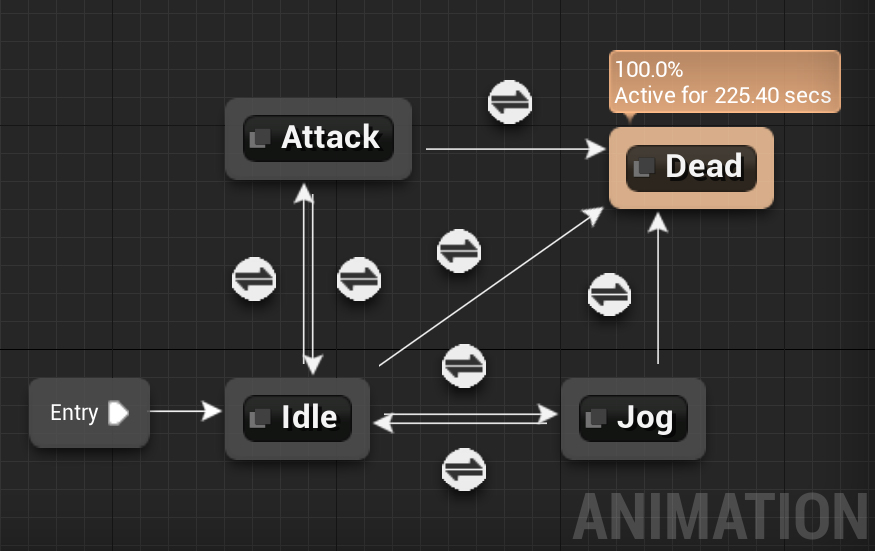
\includegraphics[scale=0.6]{animGraph.png}


%=========================================================================================
\chapter{Algorytm}
\section{Sformułowanie problemu}
Zaprogramowanie sztucznej inteligencji tak, aby zarządzała pozycjami jednostek dotyczy szczególnie analizy pozycji zapisanych przez silnik pod postacią wektorów trójwymiarowych. Dla uproszczenia możemy przyjąć, że świat gry jest dwuwymiarową mapą, co jednak nie zmienia diametralnie rozwiązań, gdyż ostatecznie operacje na wektorach wyglądają niemalże tak samo. Jednak dla prostszej analizy problemu zrezygnowałem w moim projekcie z urozmaiconych wysokości terenu - czyli trzeciego wymiaru - w poziomie gry.

Jak zaznaczyłem na wstępie - w rozdziale 'Zarys problemu pracy' - pozycje jednostek w grach RTS decydują o ich przetrwaniu oraz o przewadze w ogólnej walce. Pozycja jednostki przekłada się pośrednio na ilość jej punktów życia, a punkty te z kolei - na możliwość dłuższego zadawania obrażeń i stanowienia zagrożenia dla jednostek przeciwnika.

Algorytm, o którym mowa wywoływany jest wielokrotnie podczas każdej sekundy. Ma on za zadanie zdecydować na podstawie danych wejściowych, jaką akcję jednostka powinnna wykonać w danej chwili. Poniżej wymienione są możliwe akcje:
\begin{itemize}
\item[--] akcja ofensywna - podążanie w kierunku wrogiej armii, aż znajdzie się cel do ataku,
\item[--] atak, w przypadku braku śmiertelnego zagrożenia,
\item[--] ucieczka, w przypadku wykrycia zagrożenia śmiercią, aż do czasu pełnego wyleczenia jednostki,
\item[--] walka aż do śmierci w przypadku braku szansy na ucieczkę.
\end{itemize}

W niniejszym rozdziale umieszczone są fragmenty kodu z funkcjami używanymi przez ogólny algorytm sztucznej inteligencji gry. Fragmenty te to zazwyczaj pojednycze funkcje, które zostały napisane używając powszechnie stosowanych konwencji w branży tworzenia gier takich jak:
\begin{itemize}
\item[--] nazwy funkcji i zmiennych w notacji wielbłądziej,
\item[--] nazwy funkcji i zmiennych w języku angielskim zgodnie z zasadami samodokumentującego się kodu,
\item[--] komentarze w języku angielskim,
\item[--] typowe wcięcia kodu.
\end{itemize}

%=========================================================================================
\section{Dane wejściowe i wyjściowe}
\subsection{Dane algorytmu}
Danymi wejściowymi dla algorytmu w projekcie najprościej mówiąc jest obecny stan gry. Kluczowe tablice - 'PlayerUnits' oraz 'AIUnits' - zawierające obiekty klasy 'MyCharacter' umieszczone zostały w klasie MyGameMode dziedziczącej po natywnej klasie C++ - 'GameMode'. 

\begin{lstlisting}[language=C++, backgroundcolor=\color{black!5}, basicstyle=\footnotesize, caption=Klasa AMyGameMode.h.]
   class AMyCharacter;

UCLASS()
class SALWARTS_API AMyGameMode : public AGameMode
{
	GENERATED_BODY()

public:
	UPROPERTY(EditAnywhere, BlueprintReadWrite, Category = Units)
	TArray<AMyCharacter*> PlayerUnits;

	UPROPERTY(EditAnywhere, BlueprintReadWrite, Category = Units)
	TArray<AMyCharacter*> AiUnits;
};
\end{lstlisting}



Ponieważ każda gra w Unreal Engine 4 musi posiadać ustawiony dokładnie jeden obiekt tej klasy, prostym sposobem na przechowywanie danych, które muszą być dostępne z wielu miejsc w projekcie jest wykorzystanie mechanizmu dziedziczenia i dopisanie potrzebnych zmiennych w dziedziczącej klasie. Zarówno z poziomu Blueprint jak i C++ posiadamy dostęp do globalnych dla projektu obiektów takich jak: 
\begin{itemize}
\item[--] obecnego ustawionego trybu gry (dziedziczy po AGameMode),
\item[--] obecnego ustawionego kontrolera gracza (dziedziczy po APlayerController),
\item[--] instancji gry, nazwy gry itp,
\end{itemize}
a co za tym idzie, posiadamy też dostęp do zmiennych zadeklarowanych w tych klasach. 

Podczas instancjonowania każdej jednostki jest ona dodawana do odpowiedniej z dwóch tablic: PlayerUnits lub AiUnits, z których później algorytm sztucznej inteligencji może korzystać.

\subsection{Dane z urządzeń wejścia/wyjścia}
Komunikacja gracza z programem możliwa jest tylko przy pomocy myszki i klawiatury. Obsługa tych urządzeń zgodnie ze specyfikacją silnika jest umieszczona w klasie 'PlayerController'. W naszym projekcie funkcję assetu tego rodzaju pełni klasa Blueprint 'BP\_CameraPawnController' dziedzicząca właśnie po klasie 'PlayerController'. Zawarta w niej jest obsługa podstawowych przycisków używanych w grze: 

\begin{itemize}
\item[--] lewy przycisk myszy - po wciśnięciu i przytrzymaniu pozwala rysować prostokątu służący do zaznaczania przyjaznych jednostek,
\item[--] prawy przycisk myszy - wciśnięcie nakazuje zaznaczonym jednostkom przemieścić się w miejsce kursora,
\item[--] klawisz ,,F" - wciśnięcie tworzy nową jednostkę gracza w miejscu kursora
\item[--] klawisz ,,G" - wciśnięcie tworzy nową jednostkę komputera w miejscu kursora
\item[--] klawisz ,,B" - po przygotowaniu pola bitwy poprzez utworzenie jednostek gracza i komputera, wciskamy ten klawisz, aby rozpocząć bitwę
\item[--] klawisz 'C' - gdy wciśniemy go przed wydaniem jednostkom rozkazu poruszania się (prawy przycisk myszy), jednostki są w stanie agreswnym, co oznacza, że przerwą rozkaz poruszania się, gdy tylko napotkają jednostkę przeciwnika, na rzecz ataku.
\end{itemize}
%==================================================================================
\section{Propozycje rozwiązania problemu szukania najkrótszej drogi ucieczki}

Przed implementacją ostatecznego algorytmu rozważyłem kilka podejść do rozwiązania problemu znajdowania najkrótszej drogi ucieczki dla jednostki. Powodem jest znalezienie możliwie najwydajnieszego rozwiązania przy zachowaniu intuicyjnego dla człowieka zachowania sztucznej inteligencji. Jest to szczególnie ważne, ponieważ algorytm musi być wywoływany dla każdej z wielu zinstancjowanych jednostek w funkcji \texttt{\texttt{Tick}()}, a więc wiele razy na sekundę. Dla uproszczenia problemu rozważmy tylko algorytmy zachłanne - próbujmy znaleźć najlepsze rozwiązanie tylko dla danej chwili.

%====
\subsection{Przybliżenie pojedynczym okręgiem}
Jednym z uproszczonych rozwiązań dla znalezienia najkrótszej drogi ucieczki jest przybliżenie zbioru jednostek wrogich znajdujących się w promieniu zagrożenia do jednego - większego - okręgu lub elipsy. Jest to szczególnie proste rozwiązanie z punktu widzenia optymalizacji - złożoność obliczeniowa wyniesie O(n), gdzie 'n' będzie ilością wrogich jednostek w zasięgu. Wadą będzie niska dokładność i mało rzetelności w imitacji zachowań ludzkich. W niektórych przypadkach algorytm zachowałby się całkowicie nieintuicyjnie.
Zalety:
\begin{itemize}
\item[--] prosta implementacja,
\item[--] dobra optymalizacja,
\item[--] złożoność obliczeniowa O(n),
\end{itemize}
Wady:
\begin{itemize}
\item[--] efekt tego rozwiązania dobry tylko w szczególnych przypadkach,
\item[--] nieintuicyjne zachowanie sztucznej inteligencji.
\end{itemize}

%====
\subsection{Zmniejszona ilość dostępnych wektorów ucieczki}
Możemy zaproponować inne rozwiązanie - bardziej zbliżone do numerycznego podejścia. Jeżeli założymy określoną, skończoną ilość dostępnych wektorów ucieczki, złożoność algorytmu nie zwiększy się znacznie, a jego dokładnością możemy manipulować. 

Każda jednostka może uciekać w dowolnym kierunku który możemy opisać kątem α, gdzie:
α e <0°,360°>.
Wybór liczby potencjalnych wektorów ucieczki 'n' spowoduje podział poziomej płaszczyzny co 360°/n.

Przykład:
Jeżeli n = 6, to istnieje tylko 6 wektorów, spośród których możemy wybrać jeden - optymalny, wystarczy, że dla każdego z nich obliczymy drogę ucieczki (droga w kierunku punktu przecięcia wektora z wszystkimi (!) okręgami) i wśród wyników znajdziemy najmniejszy. Po zaledwie sześciu iteracjach otrzymamy przybliżony wektor z dokładnością do 1/6 * 360° = 60°

W tym miejscu potrzebnym jest zdefiniowanie prostej przechodzącej przez lokację zagrożonej jednostki, o kierunku zadanym przez sprawdzany wektor. Każda iteracja takiego algorytmu polega na sprawdzeniu wszystkich punktów przecięcia tej prostej z okręgami, które są promieniami zagrożenia. Zadaniem algorytmu jest porównać wszystkie odległości między lokacją jednostki, a punktami przecięć. Jako drogę ucieczki wzdłóż sprawdzanego wektora uznajemy najdłuższą z tych odległości. Złożoność takiego algorytmu dla podziału na 'n' wrogich widocznych jednostek wyniesie O(n). W tym rozwiązaniu jesteśmy ograniczeni do pewnej dokładości - z tego powodu zrezygnowałem z niego - zastosowane rozwiązanie okazało się być wydajniejesze i dokładniejsze.

%==============================================================================
\subsection{Odniesienie tylko do najbliższego zagrożenia}
Jest to najwydajniejszy sposób, niosący jednak za sobą bardzo duże wady związane z efektywnością. Polega on na tym, że ignorujemy wszelakie zagrożenia poza tym, które ma największą wagę - tzn, jest najbliżej atakowanej jendostki. Rozwiązanie to będzie niezwykle sprawne, jeżeli wykluczymy nawet najmniejszą możliwość okrążenia przez wrogie jednostki. Bowiem w przypadku drobnego nawet okrążenia, ucieczka jednostki może odbywać się cały czas w promieniu zagrożenia od jednostek umiejscowionych dalej, gdzie może nawet pojawić się większe zagrożenie na wskutek większego zagęszczenia jednostek wrogich.
%==============================================================================
\subsection{Uwzględnienie wagi zagrożenia}
Poprzedni sposób można rozszerzyć tak, aby nie tylko jedna, ale każda jednostka miała swoją wagę zagrożenia. Waga takiego zagrożenia mogłaby zależeć od kilku typowych dla gier RTS atrybutów jednostek:
\begin{itemize}
\item[--] zadawanych obrażeń,
\item[--] szybkości ataku,
\item[--] zasięgu ataku,
\item[--] obrony - czyli zmniejszenia otrzymywanych obrażeń,
\item[--] szybkości ruchu,
\item[--] obrażeń zadawanych obszarowo, zamiast jednostkowo.
\end{itemize}
Problem przydzialania wagi zagrożenia zróżnicowanym jednostkom jest jednak bardzo trudny lub raczej niemalże niemożliwy do idealnego rozwiązania przy tak wielu zmiennych. Zachowanie balansu pomiędzy różnymi rodzajami jednostek w rzeczywistości wręcz nie jest możliwe i ostatecznie tylko przy pomocy testowania i sukcesywnych zmian bylibyśmy w stanie osiągnąć zadowalające rozwiązanie. 
Jednak dla uproszczenia problemu w projekcie niniejszej pracy występuje tylko jeden - ten sam rodzaj jednostki zarówno dla gracza jak i komputera. Oznacza to sprowadzenie wagi zagrożenia tylko do dystansu pomiędzy jednostkami ponieważ to tak naprawdę jedyny aspekt, którym poszczególne jednostki się różnią.

Problem znalezienia wektora ucieczki najpierw polega na znalezieniu wektora środka zagrożenia. Gdy odejmiemy wektor obecnej pozycji jednostki x od wektora środka zagrożenia z, to otrzymamy wektor ucieczki u.

$$\vec u = \vec x - \vec z   $$

Szukanie wektora środka zagrożenia w przypadku tego rozwiązania jest poniekąd podobne do szukania środka ciężkości figury geometrycznej. Jeżeli założymy równe masy wszystkich punktów figury, wzór wtenczas byłby następujący:

$$\vec z = \dfrac{\sum_{n=0}^{N}  \vec j_n}{N},   $$ 

gdzie N oznacza ilość wszystkich punktów, a j wektor poszczególnych punktów figury. Zauważmy, że możemy potraktować jednostki jako punkty w przestrzeni o różnej wadze. Spróbujmy teraz uwzględnić wagi każdego z kolejnych punktów przy wyliczaniu sumy. Waga każdej wrogiej jednostki powinna być tym większa im bliżej się ona znajduje. Wagę (importance) zatem przedstawmy jako odwrotność dystansu od pozycji naszej jednostki (x) do pozycji jednostki wrogiej (j).

$$ importance = \dfrac{1}{|\vec x - \vec j|} $$

Gdy w kolejnych iteracjach obliczania sumy uwzględnimy wagę, otrzymamy:

$$\vec z = \dfrac{\sum_{n=0}^{N}  {importance * \vec j_n}}{N},   $$

Aby jednak waga każdej jednostki była skorelowana z ilością wszystkich jednostek, należy utworzyć mnożnik. Mnożnik ten będzie tym mniejszy im więcej wszystkich jednostek posiadamy w zasięgu i będzie zależny od sumy wszystkich wag. Będzie on oznaczał jak bardzo dana waga jest istotna na tle wszystkich innych wag. Nazwijmy wszystkie wagi jako ,,totalImportance", a mnożnik jako ,,multiplier". Wtedy mnożnik będzie ilorazem ilości jednostek i sumy ich wag:

$$ multiplier = \dfrac{N}{totalImportance} $$

Zmienną ,,totalImportance" musimy niezależnie obliczyć sumując wszystkie wagi, a gdy to zrobimy powinniśmy uwzględnić ją we wzorze końcowym na środek zagrożenia:

$$\vec z = \dfrac{\sum_{n=0}^{N}  {multiplier + importance * \vec j_n}}{N},   $$

Rozwiązanie to wybrałem jako odpowiednie do implementacji w projekcie. Głównym powodem jest pożądane zachowanie sztucznej inteligencji imitujące zachowanie człowieka. Równie ważne jest, iż ten algorytm posiada relatywnie niską złożoność obliczeniową - O(N), gdzie N oznacza ilość jednostek stanowiących zagrożenie.

%==============================================================================
\subsection{Idealne analityczne rozwiązanie}

Czy idealne rozwiązanie jest takim, którego potrzebujemy?
Jeżeli dana jednostka jest w stanie zagrożenia od więcej niż jednej jednostki wrogiej, to najkrótsza droga ucieczki musi przebiegać przez punkt przecięcia się okręgów oznaczających zasięg ataku wrogich jednostek. Jest to związane ze znalezieniem wszystkich punktów przecięć tych okręgów, a następnie znalezienie najbliżeszego z tych punktów względem nas.

Wraz z dodaniem kolejnych widocznych wrogów, złożoność obliczeniowa znalezienia kolejnych punktów przecięcia rośnie tak, jak suma ciągu arytmetycznego o różnicy równej 1. Dzieje się tak, ponieważ dla każdej kolejnej jednostki o numerze 'n' musimy obliczyć jej punkty przecięcia z pozostałymi widocznymi już wrogami (których łącznie jest n-1). Wzór na sumę takiego ciągu przedstawiony jest następująco: 

$$\sum\limits_{k=1}^n k = \frac{n(n+1)}{2}$$

Złożoność obliczeniowa wyszukiwania idealnego punktu do ucieczki w zależności od ilości istniejących jednostek będzie zatem kwadratowa. W przypadku gry RTS jest to niedopuszczalane, jako że optymalizacja jest sprawą kluczową.

%==============================================================================
\subsection{Zastosowane rozwiązanie - odwrotna średnia ważona dla wektorów - funckja GetMiddleOfEnemies()}

Zanim jednostka zdecyduje, w jakim kierunku powinna uciekać, musi ona poznać obecny środek zagrożenia. Gdy go pozna, wystarczy, że będzie uciekać, w kierunku przeciwnym do niego. W projekcie funkcją odpowiedzialną za znalezienie środka zagrożenia jest GetMiddleOfEnemies().

\begin{lstlisting}[language=C++, backgroundcolor=\color{black!5}, basicstyle=\footnotesize, caption=Funkcja GetMiddleOfEnemies() w klasie AMyCharacter]
FVector AMyCharacter::GetMiddleOfEnemies() {
	FVector middleOfEnemies = FVector::ZeroVector;
	float totalImportance = 0;		
	float totalDistance = 0;
	float importance = 0;

	for (int i = 0; i < VisibleUnits.Num(); i++) {
		float distance = FVector::Dist(
		    GetActorLocation(), 
		    VisibleUnits[i]->GetActorLocation()
		);
		importance = 1 / distance;
		totalImportance += importance;
	}

	float multiplayer = VisibleUnits.Num() / totalImportance;
	//useful for in-editor debugging
	GEngine->AddOnScreenDebugMessage(-1, 20.0f, FColor::Yellow, 
	    FString::Printf(TEXT("%f"), totalImportance));
	GEngine->AddOnScreenDebugMessage(-1, 20.0f, FColor::Green, 
	    FString::Printf(TEXT("%f"), multiplayer));


	for (int i = 0; i < VisibleUnits.Num(); i++) {
		float distance = FVector::Dist(GetActorLocation(), 
		    VisibleUnits[i]->GetActorLocation());

		importance = 1 / distance;

		middleOfEnemies += 
		    (importance * multiplayer) *  
		    VisibleUnits[i]->GetActorLocation();
	}

	
	if (MyMiddelOfEnemiesActor)
	{
		MyMiddelOfEnemiesActor->SetActorLocation(middleOfEnemies 
		    / VisibleUnits.Num());
	}
	 return middleOfEnemies / VisibleUnits.Num();
}
\end{lstlisting}

Algorytm w niej zawarty jest skonstruowany został na podstawie wzoru na szukanie środka masy punktów opisanych wektorami z tą różnicą, że każdemu elementowi przypisujemy wagę tym większą, im mniejsza jest jego odległość od wywołującego funkcję aktora. Z tego powodu wynik tego algorytmu nazwałem ,,odwrotną średnią ważoną dla wektorów". Po wywołaniu tej funkcji na aktorze będącym instacją klasy AMyCharacter algorytm zadziała następująco:
najpierw dla każdej wrogiej jednostki z tablicy widocznych wrogów - ,,VisibleUnits" - obliczana jest jej waga zagrożenia. Waga ta, jest odwrotnością odległości wroga od naszej jednostki. Odległość tą otrzymamy wołając statyczną funkcję z wbudowanej do silnika klasy FVector:

\begin{lstlisting}[language=C++, backgroundcolor=\color{black!5}, basicstyle=\footnotesize, caption=Deklaracja funkcji Dist() w klasie FVector]
static float Dist
(
    const FVector & V1,
    const FVector & V2
)
\end{lstlisting}
Wartości wszystkich wag sumowane są i zapisywane w zmiennej typu float: totalImportance. Będzie ona potrzebna, aby odpowiednio przeskalować powstały później wektor. Następnie znajdujemy iloraz ilości widocznych wrogów przez sumę wszystkich wag i zapisujemy wynik w zmiennej typu float nazwanej Multiplier. Jej wartość posłuży nam, aby odpowiednio przeskalować wagę każdej jednostki.

Teraz zadaniem algorytmu jest zsumowanie wszystkich wektorów reprezentujące pozycje widocznych wrogów w świecie gry z uwzględnieniem wagi każdego z nich oraz mnożnika, który przeskaluje każdy z tych wektorów tak, aby ich waga nie wpływała w tym miejscu na długość wektora obecnie dodawanego do sumy.
\begin{lstlisting}[language=C++, backgroundcolor=\color{black!5}, basicstyle=\footnotesize, caption=Pętla sumująca wektory pozycji wrogów z uwzględnieniem ich wag]
for (int i = 0; i < VisibleUnits.Num(); i++) {
    float distance = FVector::Dist(GetActorLocation(), 
        VisibleUnits[i]->GetActorLocation());
	importance = 1 / distance;
	middleOfEnemies += 
	    (importance * multiplayer) *  
	    VisibleUnits[i]->GetActorLocation();
}
\end{lstlisting}

Zgodnie ze wzorem na środek ciężkości figury geometrycznej o punktach masy oznaczonych kolejnymi wektorami u, suma wszystkich wektorów zostaje ostatecznie podzielona przez ich ilość:

$$\vec v = \dfrac{\sum_{n=0}^{N}  \vec u_n}{N}   $$

Tak samo w naszym przypadku, gdy otrzymamy sumę wektorów (mimo, że mają różne wagi) musimy podzielić ją przez ich ilość.
\begin{lstlisting}[language=C++, backgroundcolor=\color{black!5}, basicstyle=\footnotesize, caption=Wartość zwracana funkcji GetMiddleOfEnemies();]
return middleOfEnemies / VisibleUnits.Num();
\end{lstlisting}

Zanim funkcja zwróci odpowiednią wartość, ustawiana jest pozycja komponentu ,,MyMiddelOfEnemiesActor". Jest to drobny krążek widoczny w świecie gry użyty do celów debugowania. Dzięki niemu zobaczyć możemy punkt zwracany przez funkcję.

\begin{lstlisting}[language=C++, backgroundcolor=\color{black!5}, basicstyle=\footnotesize, caption=Ustawienie pozycji komponentu MyMiddelOfEnemiesActor w funkcji GetMiddleOfEnemies();]
if (MyMiddelOfEnemiesActor)
{
	MyMiddelOfEnemiesActor->SetActorLocation(
	    middleOfEnemies / VisibleUnits.Num());
}
\end{lstlisting}

%==============================================================================
\section{Analiza czasu i decyzja o ucieczce}
\subsection{Przedstawienie problemu ucieczki jednostki}
W projekcie każda jednostka musi poprawnie oceniać swoje szanse na przeżycie, tak, aby jednostka narażona na pewną śmierć nie uciekała redundantnie, ale walczyła aż do śmierci i przynosiła zysk w bitwie dopóki jest w stanie zadawać obrażenia wrogom.

Potrzebna jest zatem ocena czy czas, jaki jednostka jest w stanie przeżyć jest mniejszy lub równy czasowi, którego ta jednostka potrzebuje na ucieczkę.

\begin{lstlisting}[language=C++, backgroundcolor=\color{black!5}, basicstyle=\footnotesize, 

\end{lstlisting}


W projekcie służy do tego funkcja GetCurrentSurvivalTime() umieszczona w klasie \texttt{AMyCharacter.cpp}. Przy jej pomocy każda jednostka ocenia czas ucieczki na podstawie dwóch zmiennych typu float: CurrentHP oznaczającej obecną ilość punktów życia oraz damageReceivedPerSecond, oznaczającej ilość traconych punktów życia na sekundę. Zmienna damageReceivedPerSecond jest obliczana jako suma obrażeń na sekundę otrzymywanych od każdej z jednostek będącej w zasięgu instancji klasy AMyCharacter. Aby otrzymać pozostały czas przetrwania, musimy podzielić CurrentHP przez damageReceivedPerSecond. Obliczenia te obrazuje kod funkcji:

\begin{lstlisting}[language=C++, backgroundcolor=\color{black!5}, basicstyle=\footnotesize, caption=Funkcja GetCurrentSurvivalTime w klasie \texttt{AMyCharacter.cpp}.]
    float AMyCharacter::GetCurrentSurvivalTime() {
		float damageReceivedPerSecond = 0;
		// add damage done by single unit to sum, 
		// all given values are in seconds
		for (int i = 0; i < VisibleUnits.Num(); i++) { 
			damageReceivedPerSecond += VisibleUnits[i]->DamagePerAttack /
				(VisibleUnits[i]->CooldownBetweenAttacks + 
				    VisibleUnits[i]->AttackDuration);
		}
		return CurrentHp / damageReceivedPerSecond;
	}
\end{lstlisting}

Jako, że wszystkie jednostki są jednakowe, to mają też jednakowy zasięg ataku. Stąd wynika, że jeżeli jedna jednostka jest w zasięgu atatku drugiej, to druga musi być w zasięgu pierwszej. Wykorzystałen ten fakt aby uprościć kod i użyć w powyższej funkcji tablicy jednostek będących w zasięgu ataku - VisibleUnits[] - jako tablicy jednostek wrogich stanowiących zagrożenie. Jeżeli jednostki nie byłyby indentyczne, wymagałoby to, przechowywania w osobnej - dodatkowej - tablicy tych wrogów, w których zasięgu jesteśmy, niezależnie czy oni są w naszym.

Kolejną ważną wartością w algorytmie obok pozostałego czasu życia jednostki jest czas jakiego potrzebuje ona na ucieczkę. Ponieważ dysponujemy taką zmienną jak prędkość jednostki oraz jesteśmy w stanie obliczyć lub raczej - jak później zaprezentuję - numerycznie oszacować długość drogi ucieczki, czas jesteśmy w stanie obliczyć z trywialnego wzoru na prędkość:

\[ \text{prędkość jednostki} =  \dfrac{\text{droga ucieczki}}{\text{czas ucieczki}}  \]
tak więc:
\[ {\text{czas ucieczki}} =  \dfrac{\text{droga ucieczki}}{\text{prędkość jednostki}}  \]


Za obliczenie czasu ucieczki pojedynczej jednostki w projekcie odpowiedzialna jest funkcja GetCurrentEscapeTime(). Jej kod widzimy poniżej: 

\begin{lstlisting}[language=C++, backgroundcolor=\color{black!5}, basicstyle=\footnotesize, caption=Funkcja GetCurrentEscapeTime w klasie \texttt{AMyCharacter.cpp}.]
	float AMyCharacter::GetCurrentEscapeTime() {
		float characterSpeed = FVector::DotProduct(GetVelocity(), 
		    GetActorRotation().Vector());
		return GetCurrentEscapeRouteLength() / characterSpeed;
	}
\end{lstlisting}

\subsection{Decyzja o ucieczce}

Jednostka podejmuje decyzje o ucieczce na podstawie dwóch funkcji: 
\begin{itemize}
\item[--] bool CheckIfShouldEscape() - funkcja ta sprawdza czy jendostka jest w stanie zagrożenia od wszystkich widocznych wrogów. Zwraca wtenczas wartość \texttt{true}, w przeciwnym razie - \texttt{false}
\item[--] bool CheckIfCanEscape() - funkcja ta ma niemalże identyczny kod, jak ta, wymieniona wyżej. Róznica polega na dodaniu zmiennej typu float - EscapeAccuracy. Na podstawie tej zmiennej oceniane jest, czy jednostka ma fizyczną możliwość ucieczki i przetrwania. Jeżeli na podstawie zagrożenia od widocznych jednostek czas na przetrwanie jest zbyt krótki, funkcja zwraca wartość \texttt{false}, co oznacza, że nie warto uciekać i jednostka powinna walczyć do śmierci. Im większa będzie wartość zmiennej EscapeAccuracy, tym bardziej ostrożnie zachowywać się będzie jednostka. W projekcie jej wartość wynosi -1,5 i może być zmieniana w oknie edycji klas Blueprint dla jednostki BP\_BasicUnit.
\end{itemize}

Sposób implementacji powyższych funkcji przedstawia fragment kodu:

\begin{lstlisting}[language=C++, backgroundcolor=\color{black!5}, basicstyle=\footnotesize, caption=Funkcje CheckIfShouldEscape i CheckIfCanEscape w klasie \texttt{AMyCharacter.cpp}.]
bool AMyCharacter::CheckIfCanEscape() {
	if (GetCurrentSurvivalTime() < GetCurrentEscapeTime())
		return \texttt{false};
	else
		return \texttt{true};
}

bool AMyCharacter::CheckIfShouldEscape() {
	if (GetCurrentSurvivalTime() + EscapeAccuracy < 
	    GetCurrentEscapeTime()) {
		return \texttt{true};
	}
	else {
		return \texttt{false};
	}
}
\end{lstlisting}

Najpierw sprawdzane jest, czy jednostka powinna uciekać, następnie dopiero czy jest w stanie uciec. Wywołanie następuje w funkcji \texttt{\texttt{Tick}()} jak przedstawia poniższy kod.:

\begin{lstlisting}[language=C++, backgroundcolor=\color{black!5}, basicstyle=\footnotesize, caption=Wywołanie funkcji CheckIfShouldEscape i CheckIfCanEscape w funkcji \texttt{\texttt{Tick}()} klasy AMyCharacter.]
if (Team == ETeam::AI && VisibleUnits.Num() > 
    0 && CheckIfShouldEscape() ) {
			if (CheckIfCanEscape()) {
				Escape();
				unitMode = UnitMode::Escaping;
			}
		}
	}
\end{lstlisting}

%=============================================================================
\chapter{Zakończenie}
\section{Test wydajności silnika}

Zgodnie z testami wydajności na czterordzeniowym procesorze o częstotliwości taktowania 3.5GHz oraz karcie graficznej GeForce GTX 970 gra osiąga stabilny wynik ponad 60 FPS (ang. Frame Per Second - klatek na sekundę) do momonetu stworzenia x jednostek. Wydajność spada jednak drastycznie w momencie, gdy jednostki zaczną się poruszać. Spowodowane jest to zastosowaniem systemu nawigacji dostępnego w silniku, który nie jest przystosowany do gier RTS i dużej ilości jednostek. Aby zachować wydajność na poziomie 30 FPS nie powinno się tworzyć łącznie więcej niż 30 jednostek. Poniższy wykres przedstawia ilość FPS jako funkcję ilości jednostek, z których wszystkie się poruszają. Został on przygotowany na podstawie uruchamiania gry na wymienionym wcześniej urządzeniu. 

\section{Samouczek }
W rozdziale tym opisane są zasady gry oraz jak wydawać rozkazy swoim jednostkom.
Po uruchomieniu gry, zgodnie z instrukcją wyświetloną na ekranie zadaniem gracza jest rozstawienie jednostek po dwóch stronach mapy - w górnej i dolnej jej części. 

Jednostki powinny być rozstawione tak, aby wrogowie nie kolidowali ze sobą i ta sama drużyna powinna zajmować jedną część mapy. Jednostki ustawiane są pod kursorem myszy po wciśnięciu odpowiedniego przycisku - ,,F" aby stworzyć jednostkę gracza i 'G', aby stworzyć jednostkę sterowaną przez AI. Po rozmieszczeniu kilku jednostek możemy rozpocząć bitwę klawiszem 'B'. Wtedy jednostki komputera zaczną atakować nasze. Od tego momentu naszym zadaniem jest sterowanie naszymi wojskami tak aby uciekać z bitwy jednostkami najbardziej rannymi oraz wysyłać jednostki z największą ilością punktów życia do ataku najsłabszych przeciwników.

Rozkazy jednostkom możemy wydawać po wcześniejszym ich zaznaczeniu przy pomocy kliknięcia lewego przycisku myszy i przeciągnięciu jej. Zaznaczonym jednostkom możemy nakazać przemieszczenie się normalnie lub ofensywnie. Ruch zwykły to po prostu bieg w kierunku miejsca, które klikniemy prawym przyciskiem myszy. Ruch ofensywny nakazujemy, gdy przed kliknięciem prawego przycisku myszy wciśniemy klawisz 'C'. Jednostki wtedy poruszać się będą normalnie, aż do momentu, gdy jakiś przeciwnik będzie w zasięgu ataku. Wtedy nastąpi atak na widocznego przeciwnika (jednego z wielu jeżeli jest ich w danym momencie więcej).

Ponieważ jednostki regenerują swoje punkty życia, jeżeli tylko zauważymy, że któraś z naszych ma maksymalną ilość i nie walczy, powinniśmy ją wysłać do walki, aby nieustannie czerpać z niej możliwie najwięcej korzyści.

\section{Zakończenie}
Projekt będący częścią niniejszej pracy umożliwia przetestowanie implementacji wcześniej opisanych teoretycznych rozwiązań. W zależności od rozstawienia jednostek możemy uzyskać dość trudne wyzwanie dla gracza, aby pokonać sztuczną inteligencję przeciwnika. Przy jednakowym początkowym rozłożeniu sił, gdy gracz nie wykonuje żadnych akcji, komputer wygrywa dzięki swoim decyzjom. Podsumowując - praca daje przykładowe rozwiązania dla problemów, które można powszechnie napotkać przy projektowaniu przeciwników komputerowych w grze RTS.

Poruszane w pracy problemy dają duży potencjał do tworzenia ścieżek rozwoju dla współczesnej sztucznej inteligencji w grach czasu rzeczywistego. Jest to niesamowicie wartościowy temat dla firm i społeczności związanych z tworzeniem gier, który może przenieść swoje zastosowania w inne branże informatyczne i przemysłowe.




\cleardoublepage
\addcontentsline{toc}{chapter}{Bibliografia}
\begin{thebibliography}{9}

\bibitem{buro} Michael Buro, \emph{Real-Time Strategy Games: A New AI Research Challenge.}, Edmonton 2003.

\bibitem{buro} Michael Buro and Timothy Furtak, \emph{RTS Games as Test–Bed for Real–Time AI Research}, Edmonton 2003.

\bibitem{marcponsen} David Churchill and Michael Buro, \emph{SORTS: A Human-Level Approach to Real-Time Strategy AI}, Edmonton 2012.

\bibitem{buro} Michael Buro, \emph{Call for AI Research in RTS Games}, 2004, \href{http://neuralnetworksanddeeplearning.com}{http://neuralnetworksanddeeplearning.com}.

\bibitem{marcponsen} Marc Ponsen, \emph{Improving adaptive game ai with evolutionary learning}, Delft 2004.

\bibitem{marcponsen} David Churchill and Michael Buro, \emph{Incorporating Search Algorithms into RTS Game Agents}, Edmonton 2012.



\end{thebibliography}

\end{document} 